\let\negmedspace\undefined
\let\negthickspace\undefined
\documentclass[journal]{IEEEtran}
\usepackage[a5paper, margin=10mm, onecolumn]{geometry}
\usepackage{lmodern} % Ensure lmodern is loaded for pdflatex
\usepackage{tfrupee} % Include tfrupee package

\setlength{\headheight}{1cm} % Set the height of the header box
\setlength{\headsep}{0mm}     % Set the distance between the header box and the top of the text

\usepackage{gvv-book}
\usepackage{gvv}
\usepackage{cite}
\usepackage{amsmath,amssymb,amsfonts,amsthm}
\usepackage{algorithmic}
\usepackage{graphicx}
\usepackage{textcomp}
\usepackage{xcolor}
\usepackage{txfonts}
\usepackage{listings}
\usepackage{enumitem}
\usepackage{mathtools}
\usepackage{gensymb}
\usepackage{comment}
\usepackage[breaklinks=true]{hyperref}
\usepackage{tkz-euclide} 
\usepackage{listings}
\usepackage{gvv}                                        
\def\inputGnumericTable{}                                 
\usepackage[latin1]{inputenc}                                
\usepackage{color}                                            
\usepackage{array}                                            
\usepackage{longtable}                                       
\usepackage{calc}                                             
\usepackage{multirow}                                         
\usepackage{hhline}                                           
\usepackage{ifthen}                                           
\usepackage{lscape}
\begin{document}

\bibliographystyle{IEEEtran}
\vspace{3cm}

\title{8.ex.7}
\author{EE24BTECH11008 - ASLIN GARVASIS}
% \maketitle
% \newpage
% \bigskip
{\let\newpage\relax\maketitle}
\renewcommand{\thefigure}{\theenumi}
\renewcommand{\thetable}{\theenumi}
\setlength{\intextsep}{10pt} % Space between text and floats

\textbf{Question : } Find the area enclosed by the parabola $4y=3x^2$ and the line $2y=3x+12$ \\

\textbf{(a) Theoretical Solution : }
\begin{enumerate}
\item \textbf{Find Points of Intersection:} \\  
    For \( x^2 = \frac{4y}{3} \):
    \[
    V_1 = \myvec{ 
    1 & 0 \\ 
    0 & 0 
    }, \quad 
    u_1 = \myvec{ 
    0 \\ 
    \frac{-2}{3} 
    }, \quad 
    f_1 = 0
    \]
    The quadratic form is:
    \[
    \myvec{ 
    x \\ 
    y 
    }^\top 
    \myvec{ 
    1 & 0 \\ 
    0 & 0 
    }
    \myvec{ 
    x \\ 
    y 
    }
    + 2 \myvec{ 
    0 & \frac{-2}{3} 
    }
    \myvec{ 
    x \\ 
    y 
    }
    + 0 = 0
    \]

    For \( 2y = 3x + 12 \):
    \[
    V_2 = \myvec{ 
    0 & 0 \\ 
    0 & 0 
    }, \quad 
    u_2 = \myvec{ 
    -1.5 \\ 
    1 
    }, \quad 
    f_2 = -12
    \]
    The quadratic form is:
    \[
    \myvec{ 
    x \\ 
    y 
    }^\top 
    \myvec{ 
    0 & 0 \\ 
    0 & 0 
    }
    \myvec{ 
    x \\ 
    y 
    }
    + 2 \myvec{ 
    -1.5 & 1 
    }
    \myvec{ 
    x \\ 
    y 
    }
    + -12 = 0
    \]

    \item \textbf{Write the two equations in matrix form:}
    \begin{itemize}
        \item From \( Q_1(x, y) \):
        \[
        \myvec{ 
        x \\ 
        y 
        }^\top 
        \myvec{ 
        1 & 0 \\ 
        0 & 0 
        }
        \myvec{ 
        x \\ 
        y 
        }
        + 2 \myvec{ 
        0 \\ 
        \frac{-2}{3} 
        }^\top 
        \myvec{ 
        x \\ 
        y 
        }
        = 0
        \]
        Simplifies to:
        \[
        3x^2-4y=0
        \]

        \item From \( Q_2(x, y) \):
        \[
        2 \myvec{ 
        -1.5 \\ 
        1 
        }^\top 
        \myvec{ 
        x \\ 
        y 
        } -12
        = 0
        \]
        Simplifies to:
        \[
        -3x + 2y - 12 = 0 \quad \text{or equivalently, } 2y = 3x +12
        \]
    \end{itemize}

    \item \textbf{Substitute \( 2y = 3x + 12 \)  into $4y =3x^2$:}
    \begin{align}
    2(3x + 12) &= 3x^2  \\
    3x^2 - 6x -24 &= 0 \\
    x^2 -2x -8 &= 0 \\
    (x-4)(x +2) &= 0
    \end{align}

    \item \textbf{Solve for \( x \):}
    \[
    x = 4 \quad \text{or} \quad x = -2
    \]

    \item \textbf{Find \( y \) for each \( x \):}
    \begin{itemize}
        \item For \( x = 4 \), \( y = \frac{3}{4}(4)^2 = 12 \)
        \item For \( x = -2 \), \( y = \frac{3}{4}(-2)^2 = 3 \)
    \end{itemize}

    \item \textbf{The intersection points are:}
    \[
    (4, 12) \quad \text{and} \quad (-2, 3)
    \]


    \item \textbf{Set Up the Integral:}  \\
    The parabola is $4y = 3x^2 \implies y = \frac{3x^2}{4}$, and the line is $2y = 3x +12 \implies y=\frac{3x+12}{2}$.  
    To calculate the area, we integrate the difference between the parabola and the line in terms of $x$, from $x = -2$ to $x = 4$:
    \begin{align}
        \text{Area} = \int_{x=-2}^{x=4} \brak{ \frac{3x+12}{2} - \frac{3x^2}{4} } \, dx.
    \end{align} \\

    \item \textbf{Evaluate the Integral:}  \\
    Expand the integral:
    \begin{align}
        \text{Area} = \int_{-2}^{4}\frac{3x+12}{2}  \, dx - \int_{-2}^{4} \frac{3x^2}{4} \, dx.
    \end{align}

    First term:
    \begin{align}
        \frac{1}{2} \int_{-2}^{4}\brak{3x+12}&= \frac{1}{2}\brak{\frac{3x^2}{2}+12x}_{-2}^{4}= 45
        \end{align}

    Second term:
    \begin{align}
        \int_{-2}^{4} \frac{3x^2}{4} \, dx &= \frac{1}{4} \int_{-2}^{4} 3x^2 \, dx = \frac{1}{4} \brak{ x^3 }_{-2}^{4} = \frac{1}{4} \cdot 72 = 18.
    \end{align}

    Now subtract:
    \begin{align}
        \text{Area} &= 45 -18 = 27
    \end{align} \\
    
\textbf{(b) Numerical Solution / Simulation : } \\

We aim to compute the integral:

\[
I = \int_{x=-2}^{x=4} \brak{ \frac{3x+12}{2} - \frac{3x^2}{4} } \, dx.
\]

using the trapzoidal trule approach. \\

    \item \textbf{Discretize the Interval:}  
    Divide the interval $[-2, 4]$ into $N = 100$ equal subintervals. The step size is:
    \begin{align}
    h = \frac{4 - -2}{N} = \frac{6}{100} = 0.06.
    \end{align}
    The discrete points are:
    \begin{align}
    x_i = -2 + i \cdot h, \quad \text{for } i = 0, 1, 2, \dots, 100.
    \end{align}
    For example:
    \begin{align}
    x_0 = -2, \quad x_1 = -1.94, \quad x_2 = -1.88, \, \dots, \, x_{100} = 4.
    \end{align}

    \item \textbf{Define the Function:}  
    The function to integrate is:
    \begin{align}
    f(x) = \frac{3x+12}{2} - \frac{3x^2}{4}.
    \end{align} \\

    \item \textbf{Establish the difference equation:} 
    
    Using the trapazoidal rule , 
    \begin{align}
    I_{n} = I_{n-1} + \frac{h}{2} \brak{ f(x_n) + f(x_{n-1})} 
      \end{align}
    where:
    \begin{enumerate}
        \item $I_n$: The approximate integral value up to the $n$-th point,
        \item $h = 0.06$: The step size,
        \item $f\brak{x_n} = \frac{3x_n+12}{2} - \frac{3x_n^2}{4}$: The function evaluated at $x_n$. \\
    \end{enumerate} 
   
      So, the integral can be approximated as, 
    \begin{align}
    \label{trap}
    I_n &= I_{n-1} + \frac{h}{2} \brak{ \brak{\frac{3x_n+12}{2} - \frac{3x_n^2}{4}} + \brak{\frac{3x_{n-1}+12}{2} - \frac{3x_{n-1}^2}{4}}} \\ 
    x_n &= x_{n-1} + h
   \end{align}
    \item \textbf{Iterative Computation:}  
    The recurrence relation is applied iteratively starting with the initial condition:
    \begin{align}
    I_0 = 0.
    \end{align}
    Each step updates $I_n$ using the values of $f(x_n)$ and $f(x_{n-1})$. \\

    \item \textbf{Final Value:}  
    After iterating up to $n = 100$, the value of the integral at the upper bound $x = 4$ is:
    \begin{align}
    I[100] &= 27
    \end{align}

\textbf {Using the difference equation \eqref{trap} we can code to simulate the area pretty easily . Choosing n = 100 we get area as 27 which verifies with the theoretical solution.}

	 \begin{figure}[h]  % The 'h' means 'here' (positioning)
    \centering  % Centers the figure
    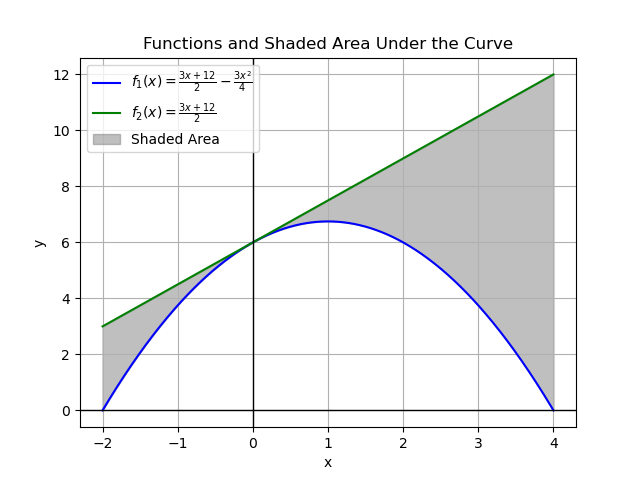
\includegraphics[width=\columnwidth]{figs/Figure_1.png}  
    \caption{Graph}
    \label{fig:example}  % Label for referencing
\end{figure}
\end{enumerate}
\end{document}
